\documentclass[11pt]{article}
\usepackage{geometry}                % See geometry.pdf to learn the layout options. There are lots.
\geometry{letterpaper}                   % ... or a4paper or a5paper or ... 
%\geometry{landscape}                % Activate for for rotated page geometry
%\usepackage[parfill]{parskip}    % Activate to begin paragraphs with an empty line rather than an indent
\usepackage{graphicx}
\usepackage{caption}
\usepackage{amssymb}
\usepackage{wrapfig}
\usepackage{amsmath}
\usepackage{epstopdf}
\DeclareGraphicsRule{.tif}{png}{.png}{`convert #1 `dirname #1`/`basename #1 .tif`.png}

\title{Playing with the E\&M Toy Model:\\A Charged Spinning Sphere}
\date{}                                           % Activate to display a given date or no date

\begin{document}
\maketitle
\section{Comparing the E\&M Analogy with Kerr}
I argued in [insert section number here] that E\&M is a strong analog to gravity.  That was a generic field theoretic argument; let's take advantage of this analogy to use electromagnetism to get some concrete predictions about gravity.  Taking the analogy as valid, we can construct a toy model to compare with Kerr.

To review, mapping gravity to electromagnetism, we can say:

\begin{align}
m &\rightarrow q   \text{ (mass becomes charge)}\\
G &\rightarrow \frac{1}{4\pi\epsilon_0} \text{ (constants switch)}\\
+ &\rightarrow - \text{ (gravity is attractive; electricity, repulsive)}
\end{align}

Then, making special relativistic considerations, we can derive necessary magnetic fields as corrections to both electricity and gravity.
\begin{figure}[h]
  \begin{center}
    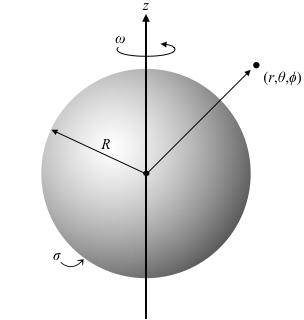
\includegraphics[scale=.65]{/Users/alexdeich/thesis/latex/figs/charged_spinning_sphere.png}
  \end{center}
  \caption{}
  \label{fig:charged_spinning_sphere}
\end{figure}

So, we're studying orbits in the Kerr spacetime, which is the consequence of a spinning mass.  Accounting for the above mapping then, we should expect the analogous E\&M system to be represented by Fig.\ref{fig:charged_spinning_sphere}:  A charged spinning sphere.  Specifically, we want to study the orbit of a charged particle near the sphere.  More to the point of this thesis, we seek how the orbits of the particles change when the spin of the central sphere changes.  The E\&M model will help us build intuition about the full gravity case.

\section{A Description of the Relevant Magnetic Vector Potential}
All quantities refer to Fig.\ref{fig:charged_spinning_sphere}.  Our system is a solid sphere of radius $R$ with constant surface charge density $\sigma$, rotating about the $z$ axis with some angular frequency $\omega$.

 The magnetic vector potential at an arbitrary point $(r,\theta,\phi)$ outside the sphere is given by $\mathbf{A} = \frac{\mu_0R^4\sigma}{3}\frac{\sin\theta}{r^2}\mathbf{\hat{\phi}}$.  The derivation for this is reproduced in Appendix [insert number].  For our purposes, it is helpful to reparameterize the vector potential with the angular momentum, $l$ and total charge $Q$ instead\footnote{This change is made using the angular momentum per unit mass, $I\omega/M$, with the moment of inertia of a sphere, $I = 2MR^2/5$.}:
 \begin{equation}\label{eq:vec_pot}
 \mathbf{A} = \frac{1}{2}\frac{\mu_0 Q l}{4\pi}\frac{\sin\theta}{r^2}\mathbf{\hat{\phi}}
 \end{equation}
The electric potential is unchanged from a static sphere: $V = \frac{Q}{4\pi\epsilon_0r}$.

It is worth stopping here and considering how this applies to the analogy of E\&M with gravity.  I have written in (\ref{eq:vec_pot}) the vector potential of the object I want to act as an analogue to a spinning mass.  The potential determines the trajectories of charged particles, so it plays the role of the metric in this analogy.  Combining (\ref{eq:vec_pot}) with the electric potential, then, the relativistic four-potential reads
\begin{equation}\label{eq:em_4_pot}
A^\mu = Q\left(
\begin{array}{c}
\frac{1}{4\pi c\epsilon_0r}\\
0\\
0\\
\frac{1}{2}\frac{\mu_0  l}{4\pi}\frac{\sin\theta}{r^2}
\end{array}
\right).
\end{equation}

We expect gravity to affect the motions of particles in the same way (up to a difference of sign).  Therefore, in order to affect particle motion in the same way as (\ref{eq:em_4_pot}), we expect the form of the $(t,\nu)$ column of the metric to take after the form of  (\ref{eq:vec_pot}).  However, a metric is necessarily a symmetric object, so any element in the $\mu,\nu$ is also in the $\nu,\mu$ position.  Therefore, we expect:

\begin{equation}\label{eq:rough_metric}
g^{\mu\nu} =
\left(
\begin{array}{cccc}
t t &0 &0 &\phi t\\
0 &\dots&0&0\\
0&0&\dots&0\\
t \phi&0&0&\phi\phi
\end{array}
\right)
\end{equation}
for some undefined $t,\phi$ elements.

So, by insisting that: 1) the metric of a spinning mass mimic the form of the potential for the spinning charged object, and 2) the metric be symmetric, we recover the $\phi$-time coupling which characteristic of Kerr spacetime.  While not terribly rigorous, I find this a satisfying way of justifying what is at first a strange quality.

\section{Particle Trajectories}
To probe the trajectory of a particle of charge $q$ near the spinning sphere, we need to look at the Lagrangian $L = \frac{1}{2}m\mathbf{v}^2 - qV + q\mathbf{v}\cdot\mathbf{A}$:

\begin{equation}\label{eq:particle_lagr}
L = \frac{1}{2}m\left(\dot{r}^2 + r\cos\dot{\theta} + r\sin^2\theta\dot{\phi}\right) - \frac{qQ}{4\pi\epsilon_0r} + \frac{\mu_0qQl}{8\pi}\frac{sin^2\theta}{r}\dot{\theta}.
\end{equation}
 
For this analysis, we restrict ourselves to the $\theta = \pi/2$ plane.  Having done this, the Lagrangian reveals two constants:  Angular momentum about the $z$ axis, $J_z \equiv \frac{\partial L}{\partial \dot{\phi}}$, and the total energy, $E$.  Rewriting the resultant equations of motion in terms of these constants is helpful in setting initial conditions.

The relevant equations of motion are
\begin{align}
\ddot{r} &= \frac{J_z}{4\pi m^2 r^3} + \frac{qQ}{4\pi\epsilon_0 m r^2} - \frac{\mu_0 q Q l}{8 \pi m^2}\left(\frac{J_z}{3r^4} - \frac{\mu_0 q Q l}{16\pi r^5}\right)\label{eq:r_eom}\\
\dot{\phi} &= \frac{J_z}{r^2m} - \frac{\mu_0qQl}{8\pi m r^3}\label{eq:ph_eom}
\end{align}

Of note is that (\ref{eq:r_eom}) has both attractive and repulsive terms, with different regimes of domination.  The electric term, $\frac{qQ}{4\pi\epsilon_0 m r^2}$, is repulsive, and so will not give bound orbits for large $r$.  However, it also grows large more slowly than the attractive magnetic terms, which depend on $1/r^4$ and $1/r^5$.  So, closed orbital motion will only occur for very close particles.

\section{Numerical Simulation}
We're interested in how changes in the sphere's angular frequency affects the orbits of particles near the sphere.  In the context of (\ref{eq:particle_lagr}) and the resulting equations of motion, (\ref{eq:r_eom}) and (\ref{eq:ph_eom}), change in angular frequency is encoded in change in the angular momentum, $l$.  While we could have left $l$ as an arbitrary function of time, $l(t)$ and found equations which depended on some $\dot{l}$ term, it is more helpful in building intuition to leave it as is and perform numerical simulations which change $l$ explicitly.

To perform the numerical simulation, (\ref{eq:r_eom}) and (\ref{eq:ph_eom}) were written with all constants unity\footnote{if this worries you, it's really just lazy nondimensionalization--- it prevents us from solving for any helpfully paramterized initial conditions, but it gives a quick picture of the behavior of the system} and plugged into a Python ODE solver, \texttt{odeint} in the \texttt{scipy} scientific computation package.



As a first test case with $l = 0$, we retrieve a closed elliptical orbit (Fig.\ref{fig:closed_em_orbit})


When $l$ takes a small value, the system exhibits precession about the sphere (Fig. \ref{fig:constant_l_em_orbit}).




In an exaggerated model analogy of a pulsar glitch, we step-function $l$ to instantaneously increase tenfold (Fig. \ref{fig:step_func_em_orbit})


Finally, we get a little funky with $l = \sin(t)$ (Fig.\ref{fig:sin_em_orbit}).  This has some interesting and, to me at the moment, obscure behavior:  The particle initially appears bound, but as time goes on, its orbit grows and grows until the repulsive electric term dominates and the particle flies off to infinity.  It looks like there is some strange momentum transfer occurring which would be good to investigate.

\section{Applying this to Gravity}
So, this gives us some notion of what to expect for particles in Kerr geometry:  In a weak-field setting, they will exhibit precession for a mass with constant spin.  A step-function spin will give their trajectories take the intuitive kick:  Ignoring any momentum in the particle, they will be cast suddenly in a new orbit.  The sinusoidally changing spin is less helpful here as there's no field of opposite sign to repel the particle at large $r$.  Nonetheless, we can expect the particle to grow in orbit.  An interesting thing to investigate for would be some kind of resonance:  How is the orbital frequency of the particle related to the angular frequency of the mass?  Are there relationships between these frequencies which don't result in a growing orbit?
\newpage
\begin{figure}[h]
  \begin{center}
    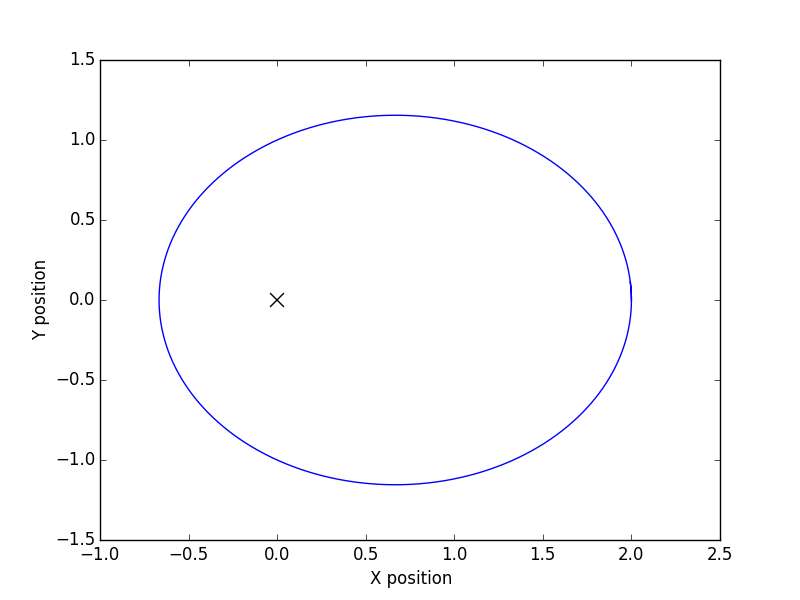
\includegraphics[scale=.5]{/Users/alexdeich/thesis/latex/figs/closed_em_orbit.png}
  \end{center}
  \caption{A charged particle orbiting a charged static sphere (the cross at the origin) exhibits closed elliptical motion.}
  \label{fig:closed_em_orbit}
\end{figure}

\begin{figure}[h]
  \begin{center}
    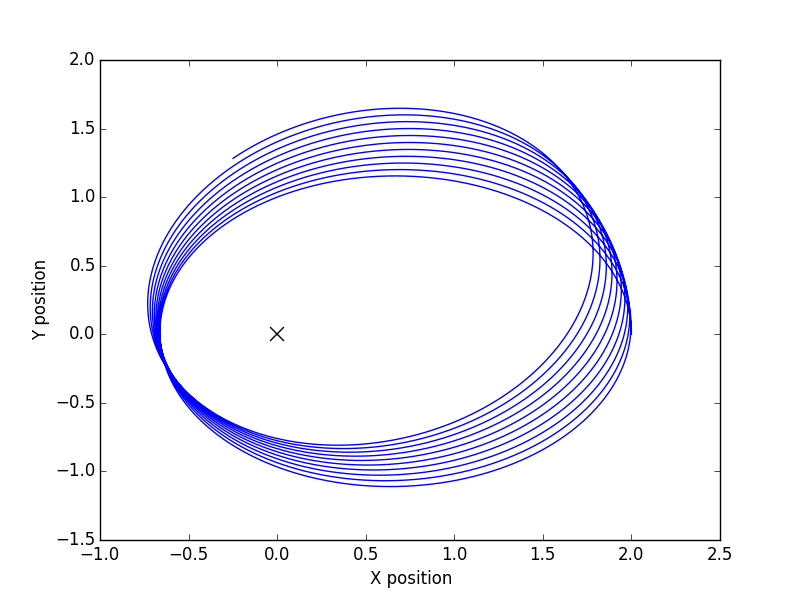
\includegraphics[scale=.5]{/Users/alexdeich/thesis/latex/figs/constant_l_em_orbit.png}
  \end{center}
  \caption{$l = 0.005$}
  \label{fig:constant_l_em_orbit}
\end{figure}

\begin{figure}[h]
  \begin{center}
    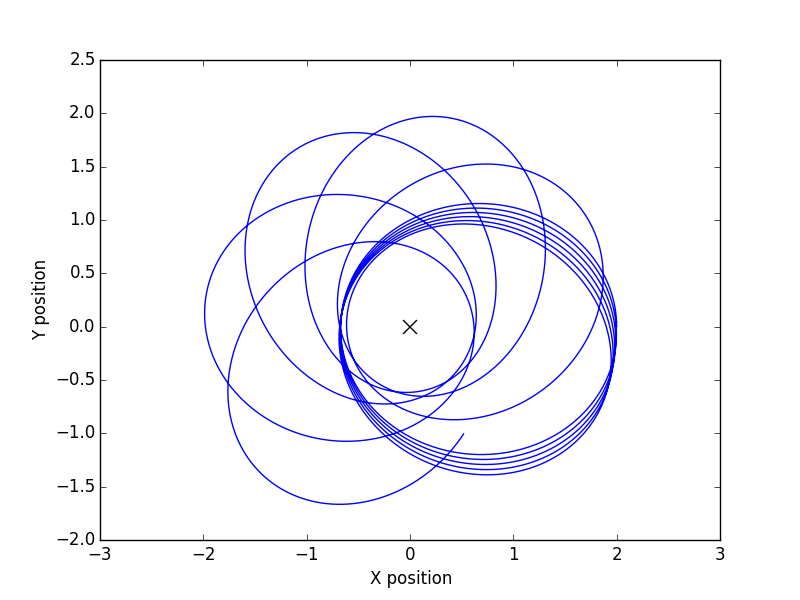
\includegraphics[scale=.5]{/Users/alexdeich/thesis/latex/figs/step_func_em_orbit.png}
  \end{center}
  \caption{$l = 0.005 \rightarrow l=0.05$.  This basically what we'd expect; the particle trajectory is just two static cases glued together.  In this case, we are assuming the particle has negligible mass, so its momentum does not affect the change in trajectory.}
  \label{fig:step_func_em_orbit}
\end{figure}

\begin{figure}[h]
  \begin{center}
    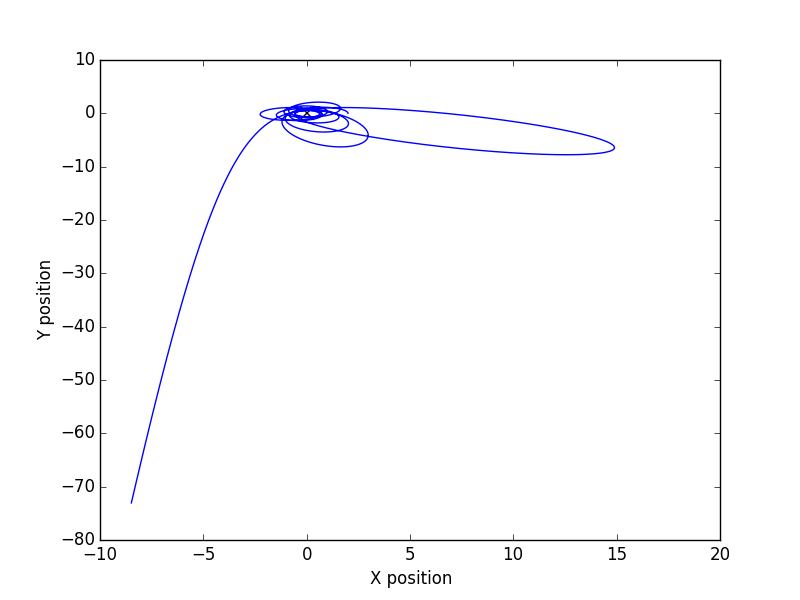
\includegraphics[scale=.5]{/Users/alexdeich/thesis/latex/figs/sin_em_orbit.png}
  \end{center}
  \caption{$l = sin(t)$}
  \label{fig:sin_em_orbit}
\end{figure}

\end{document}  